\section{Évaluation de l'hypothèse de rentabilité}
\label{section:4.5-HYPOTHESE-RENTABILITE}

	%%% Introduction / Transition.
	Dans les études précédentes, le cas d'arrêt de notre méthodologie d'annotation basée sur le \textit{clustering} interactif était conditionné à la vérité terrain.
	En effet, nous utilisions un seuil de $90$\% de \texttt{v-measure}, caractérisant une annotation dite "partielle" de la base d'apprentissage.
	Cependant, une telle référence n'est pas accessible en situation réelle car l'objectif de notre méthode est précisément de la construire cette vérité terrain.
	Nous devons donc nous intéresser à d'autres moyens pour estimer la rentabilité d'une itération supplémentaire et pouvoir ainsi définir de nouveaux cas d'arrêt pour le \textit{clustering} interactif.
	Pour cela, nous aimerions vérifier l'hypothèse suivante :
	
	%%% Formulation des hypothèses:
	\begin{tcolorbox}[
		title=\faVial~\textbf{Hypothèse de rentabilité}~\faVial,
		colback=colorTcolorboxHypothesis!15,
		colframe=colorTcolorboxHypothesis!75,
		width=\linewidth
	]
		« \textbf{
			Au cours d'une méthodologie d'annotation basée sur le \textit{clustering} interactif, il est possible d'estimer la rentabilité d'une itération supplémentaire de la méthode, et ainsi d'établir des cas d'arrêt indépendant d'une vérité terrain pour obtenir une base d’apprentissage satisfaisante.
		} » \\
		
		% Figure.
		La \textsc{Figure~\ref{figure:4.5-HYPOTHESE-RENTABILITE}} illustre cette hypothèse et l'espoir de pouvoir estimer le rapport entre le gain de pertinence obtenu et le coût nécessaire pour l'obtenir.
		%
		\begin{figure}[H]  % keep [H] to be in the tcolorbox.
			\centering
			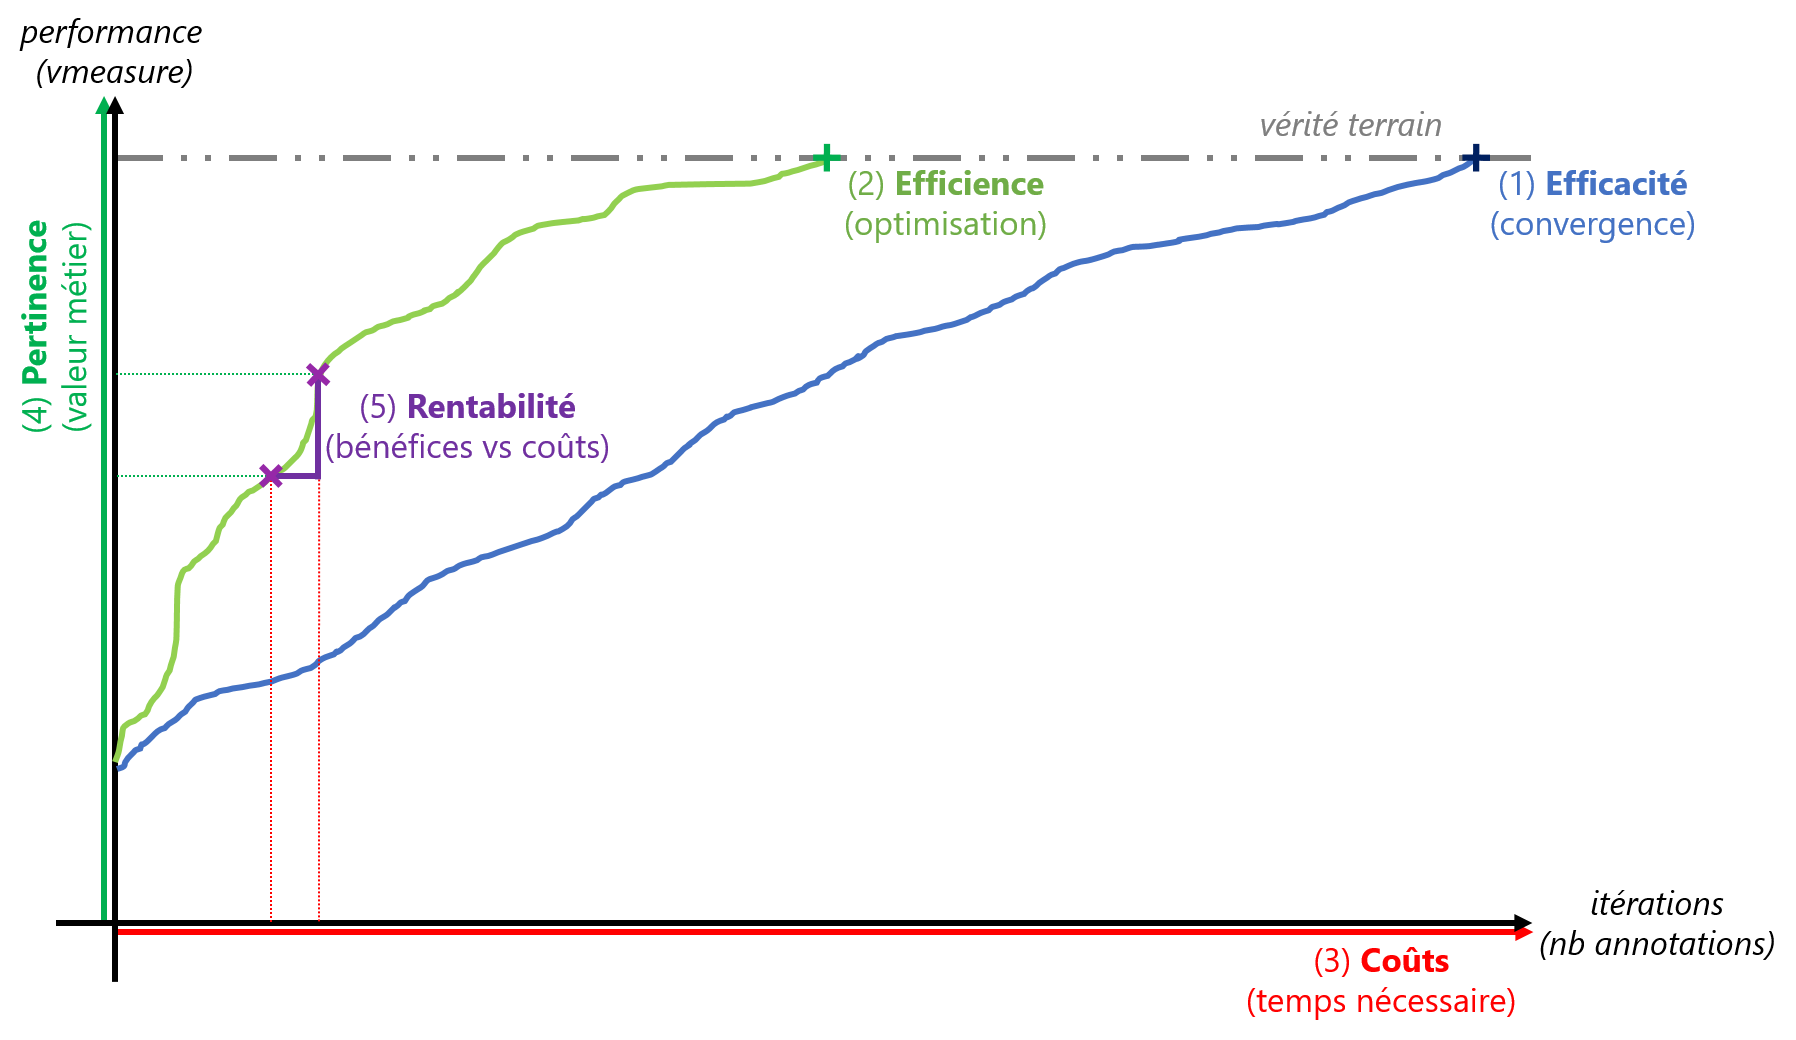
\includegraphics[width=0.95\textwidth]{figures/hypotheses-05-rentabilite}
			\caption{
				Illustration des études réalisées sur le \textit{clustering} interactif (\textit{étape 5/6}) en schématisant l'évolution de la pertinence (\textit{valeur métier évaluée par l'expert et exprimé en nombre de clusters}) d'une base d'apprentissage en cours de construction en fonction du coût temporel de la méthode (\textit{temps nécessaire à l'expert métier et à la machine}), ainsi que la rentabilité de chaque itération de la méthode (\textit{rapport entre le gain potentiel de pertinence et le coût à investir}).
			}
			\label{figure:4.5-HYPOTHESE-RENTABILITE}
		\end{figure}
	\end{tcolorbox}
		
	% Résumé de l'étude.
	Afin de vérifier cette hypothèse, nous explorons deux approches :
	\begin{itemize}
		\item l'évolution de l'\textbf{accord entre l'annotation de l'expert et le \textit{clustering}} sur lequel est basé l'échantillon d'annotation, permettant d'estimer si la machine doit encore être corrigée par l'annotateur  (cf. \textsc{Section~\ref{section:4.5.1-ETUDE-RENTABILITE-ACCORD-ANNOTATION-CLUSTERING}}) ;
		\item et l'évolution de la \textbf{différence entre deux \textit{clusterings} successifs}, permettant de mesurer s'il y a eu des changements visibles dans le partitionnement des données après l'ajout des dernières contraintes (cf. \textsc{Section~\ref{section:4.5.2-ETUDE-RENTABILITE-SIMILARITE-CLUSTERING}}).
	\end{itemize}
	
	
	%%%
	%%% Subsection 4.5.1: Étude de l'évolution d'accord entre l'annotation et le \textit{clustering}.
	%%%
	\subsection{Étude de l'évolution d'accord entre l'annotation et le \textit{clustering}}
	\label{section:4.5.1-ETUDE-RENTABILITE-ACCORD-ANNOTATION-CLUSTERING}
		
		% Objectif de l'expérience.
		Nous cherchons à trouver un cas d'arrêt du \textit{clustering} interactif ne nécessitant pas de comparaison avec une vérité terrain, et notre première intuition concerne l'étude des annotations réalisées.
		En effet, à chaque itération, l'expert annote un échantillon de contraintes dans le but de confirmer ou de corriger le \textit{clustering} de l'itération précédente.
		Or, après un nombre suffisant d'itérations, le \textit{clustering} commence à se stabiliser : il devrait donc y avoir davantage d’annotations qui confirment le \textit{clustering} que d'annotations qui le corrigent, puis n'avoir que des accords entre les annotations et le \textit{clustering}.
		Ainsi, nous allons étudier l'évolution du nombre de contraintes annotées qui approuvent le partitionnement des données obtenu et essayer d'adapter cette analyse en cas d'arrêt pour notre méthode d'annotation.
	
		%%% Protocole expérimental.
		\subsubsection{Protocole expérimental}
			
			% Axiome.
			\begin{leftBarWarning}
				Dans le cadre de cette étude, nous supposons que l'expert métier connaît parfaitement le domaine traité dans ce jeu de données, et qu'il est capable de caractériser sans ambiguïté la similitude entre deux données issues de cet ensemble.
			\end{leftBarWarning}
			
			% Pseudo-code.
			Pour résumer le protocole expérimental que nous décrivons ci-dessous, vous pouvez vous référer au pseudo-code décrit dans \textsc{Algorithme~\ref{algorithm:4.5.1-ETUDE-RENTABILITE-ACCORD-ANNOTATION-CLUSTERING-PROTOCOLE}}.
			
			\begin{algorithm}
				\KwData{jeu de données annotés (vérité terrain)}
				%
				\ForEach{jeux de données à tester}{
					\textbf{initialisation (données)}: récupérer les données et la vérité terrain \;
					\textbf{initialisation (contraintes)}: créer une liste vide de contraintes \;
					\textbf{prétraitement}: supprimer le bruit dans les données avec \texttt{prep.simple} \;
					\textbf{vectorisation}: transformer les données en vecteurs avec \texttt{vect.tfidf} \;
					\textbf{clustering initial}: regrouper les données par similarité avec \texttt{clust.kmeans.cop} \;
					\Repeat{annotation de toutes les contraintes possibles}{
						\textbf{échantillonnage}: sélectionner des contraintes avec \texttt{samp.closest.diff} \;
						\textbf{simulation d'annotation}: caractériser les contraintes grâce à la vérité terrain \;
						\textbf{intégration}: ajouter les nouvelles contraintes au gestionnaire de contraintes \;
						\textbf{rentabilité}: calculer l'accord entre l'annotation et le \textit{clustering} précédent \;
						\textbf{clustering}: regrouper les données par similarité avec \texttt{clust.kmeans.cop} \;
					}
				}
				\textbf{analyse 1}: afficher l'évolution de l'accord entre annotation et \textit{clustering} \;
				\textbf{analyse 2}: calculer la corrélation entre le score d'accord et le score de performance \;
				%
				\KwResult{discussion sur la rentabilité d'après l'accord entre annotation et \textit{clustering}}
				%
				\caption{\textit{
					Description en pseudo-code du protocole expérimental de l'étude de l'évolution d'accord entre l'annotation et le \textit{clustering}.
				}}
				\label{algorithm:4.5.1-ETUDE-RENTABILITE-ACCORD-ANNOTATION-CLUSTERING-PROTOCOLE}
			\end{algorithm}
			
			% Description de la vérité terrain.
			Nous utilisons comme vérité terrain le jeu de données \texttt{Bank Cards (v1.0.0)} : ce dernier traite des demandes les plus fréquentes des clients en ce qui concerne la gestion de leur carte bancaire.
			Il est composé de $500$ questions rédigées en français et réparties en $10$ classes (\texttt{perte ou vol de carte}, \texttt{carte avalée}, \texttt{commande de carte}, ...).
			Pour plus de détails, consultez l'annexe~\ref{annex:C.1-DATASET-BANK-CARDS}.
			
			% Description des tentatives de la méthode et du calcul de rentabilité.
			Sur ce jeu de données, nous exécutons une tentative complète
			\footnote{Tentative complète : itérations d'échantillonnage, d'annotation et de \textit{clustering} jusqu'à annotation de toutes les contraintes possibles.}
			\todo{Utiliser 'footmisc' et 'footref' pour faire des notes de bas de pages communes ? ou lien vers des conclusions ?}
			de la méthode du \textit{clustering} interactif en utilisant notre paramétrage favori, et cette tentative est répétée $5$ fois pour contrer les aléas statistiques des exécutions.
			À chaque itération, un lot de $50$ contraintes est sélectionné puis annotés en simulant l'action d'un expert métier, et nous évaluons l'accord entre ces nouvelles annotations et la proposition de partitionnement des données réalisé par le \textit{clustering} à l'itération précédente :
			\begin{itemize}
				\item il y a \textbf{accord} lorsqu'une contrainte de deux données issues d'un même \textit{cluster} est annotée \texttt{MUST-LINK}, ou lorsqu'une contrainte de deux données issues de deux \textit{clusters} différents est annotée \texttt{CANNOT-LINK} (cf. \textsc{Figure~\ref{figure:4.5.1-ETUDE-RENTABILITE-ACCORD-ANNOTATION-CLUSTERING-EXEMPLE} (1)}) ;
				\item il y a \textbf{désaccord} lorsqu'une contrainte de deux données issues d'un même \textit{cluster} est annotée \texttt{CANNOT-LINK}, ou lorsqu'une contrainte de deux données issues de deux \textit{clusters} différents est annotée \texttt{MUST-LINK} (cf. \textsc{Figure~\ref{figure:4.5.1-ETUDE-RENTABILITE-ACCORD-ANNOTATION-CLUSTERING-EXEMPLE} (2)}).
			\end{itemize}
			Nous pouvons ainsi calculer un score d'accord défini par la ratio entre le nombre d'accords et le nombre de contraintes annotées.
			Pour nous permettre de discuter de l'utilité de ce score pour prédire la stabilisation du \textit{clustering} et ainsi définir un cas d'arrêt de notre méthodologie d'annotation, nous calculons aussi le score de corrélation entre cet accord et la performance obtenu à l'aide d'une vérité terrain (la corrélation \texttt{r} de \textit{Pearson} (\cite{kirch:2008:pearson-correlation-coefficient}) est utilisée).

			\begin{figure}[!htb]
				\centering
				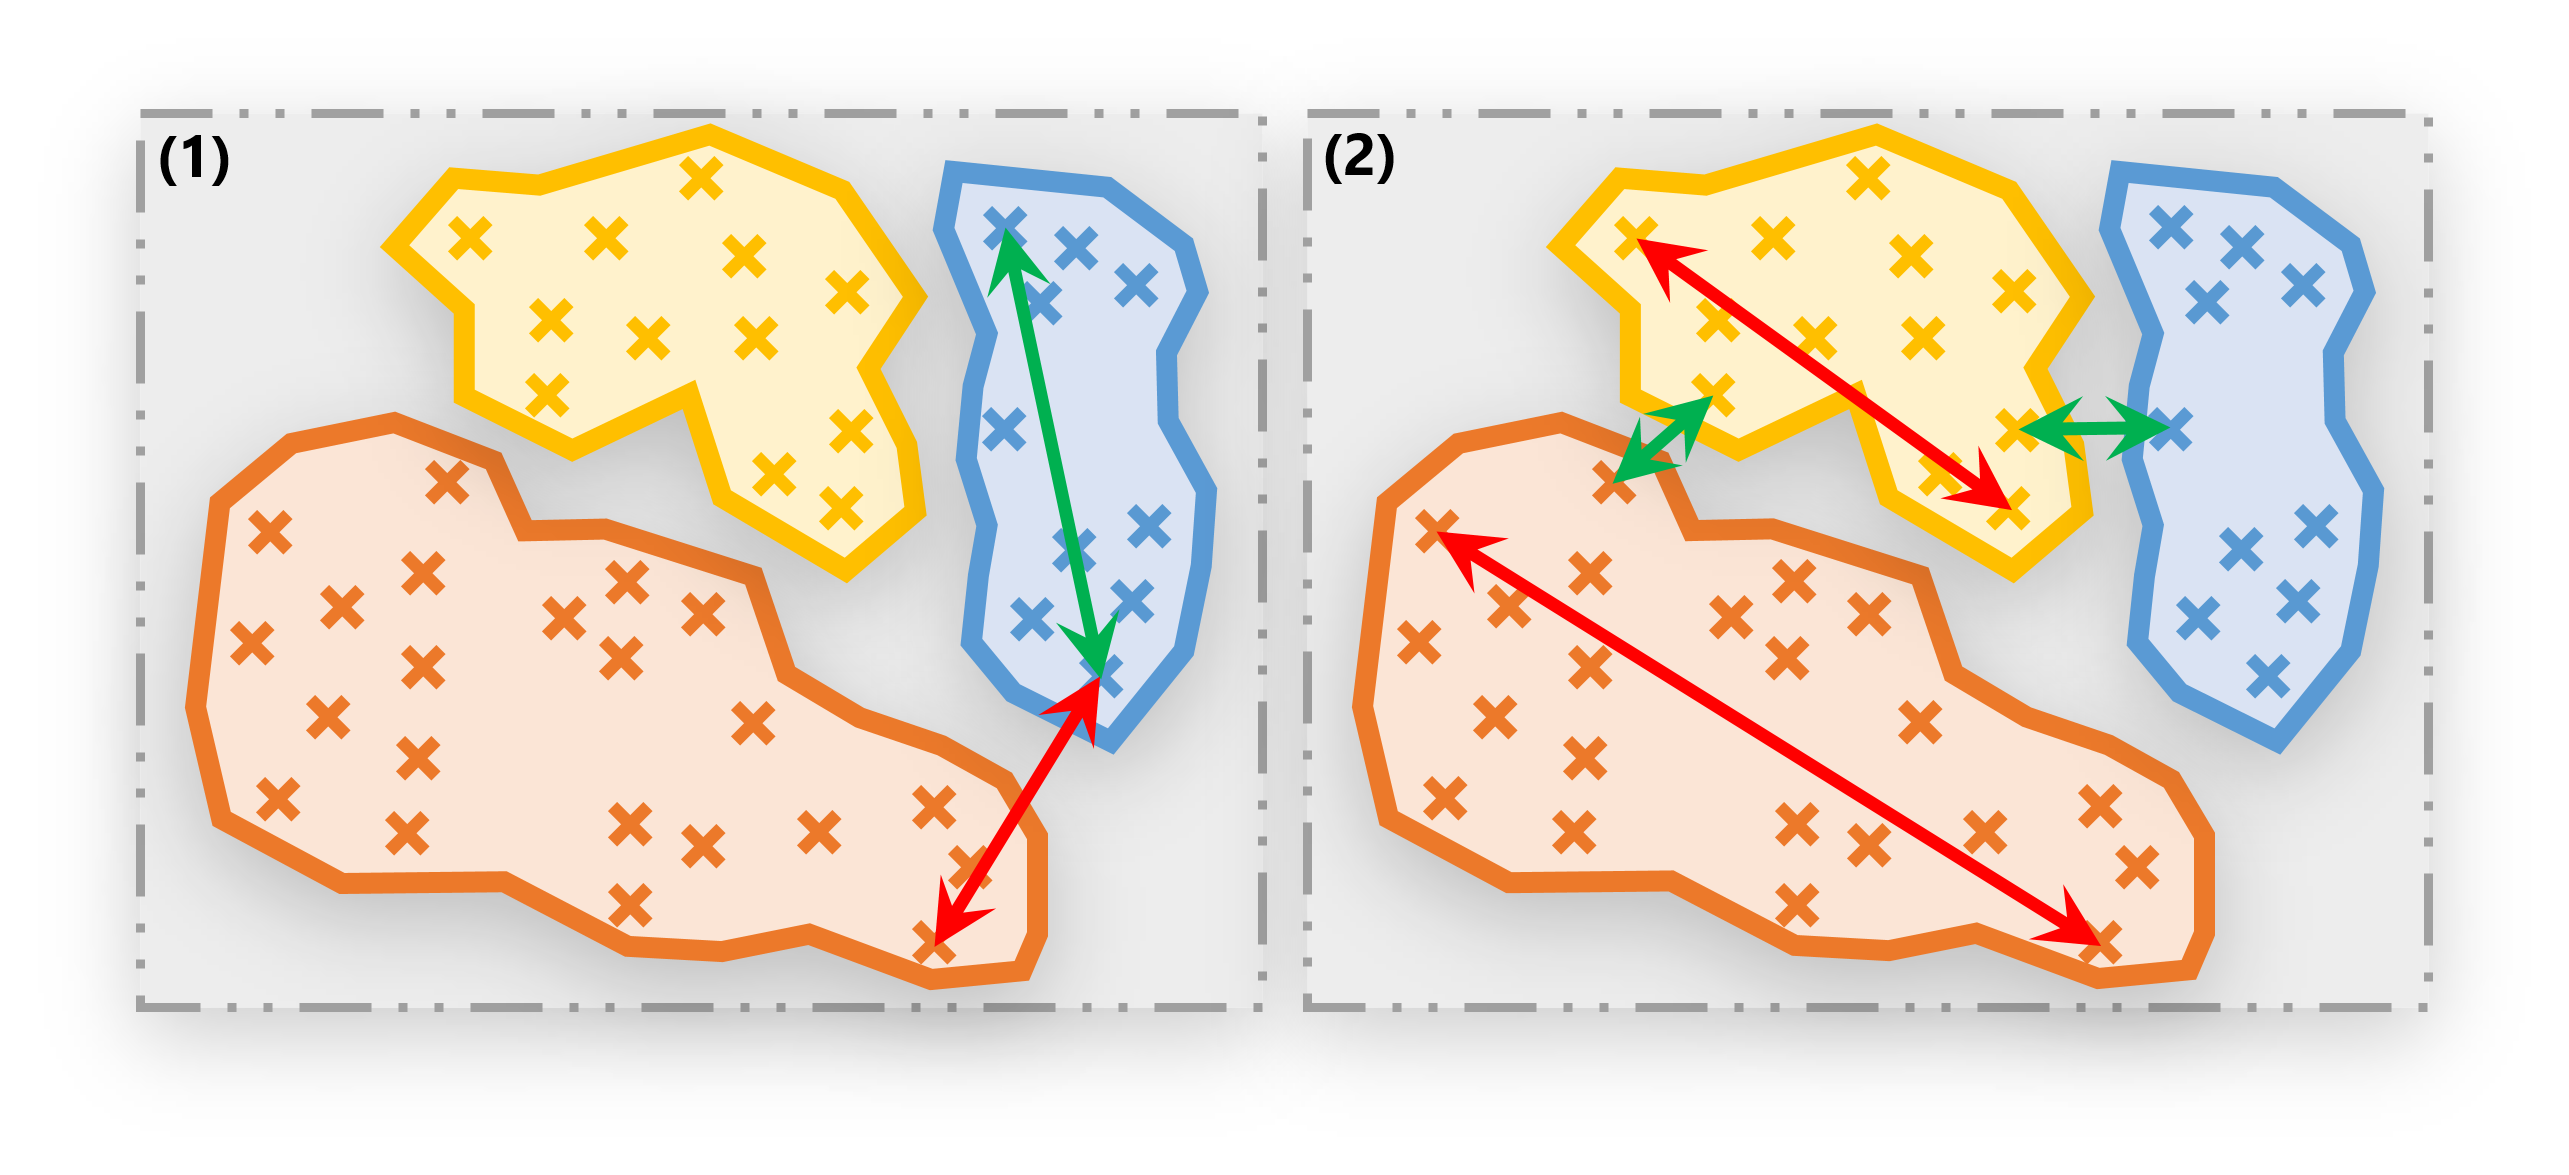
\includegraphics[width=0.7\textwidth]{figures/example-accord-annotation-clustering}
				\caption{
					Exemples d'accords et de désaccord entre les annotations d'une itération et le résultat du \textit{clustering} de l'itération précédente.
					Des contraintes \texttt{MUST-LINK} (flèches vertes) et \texttt{CANNOT-LINK} (flèches rouges) sont représentées dans deux situations : \textbf{(1)} montre des cas d'accords (\texttt{MUST-LINK} dans un même \textit{cluster}, \texttt{CANNOT-LINK} entre deux \textit{clusters} différents), et \textbf{(2)} montre des cas de désaccords (\texttt{MUST-LINK} entre deux \textit{clusters} différents, \texttt{CANNOT-LINK} dans un même \textit{cluster}).
				}
				\label{figure:4.5.1-ETUDE-RENTABILITE-ACCORD-ANNOTATION-CLUSTERING-EXEMPLE}
			\end{figure}
			
			\begin{leftBarIdea}
				Nous concentrons l'étude sur notre paramétrage favori (voir \textsc{Section~\ref{section:4.4.3-ETUDE-PERTINENCE-RESUME-AUTOMATIQUE}}).
				Cependant, afin de compléter notre discussion avec d'autres points de comparaison, nous analysons aussi les autres paramétrages implémentés, notamment les meilleurs paramétrages moyens identifiés lors de l'hypothèse d'efficience (voir \textsc{Section~\ref{section:4.2-HYPOTHESE-EFFICIENCE}}).
			\end{leftBarIdea}
			
			% Référence scripts.
			\begin{leftBarInformation}
				Les scripts de l'expérience, réalisés avec des \textit{notebooks} Python (\cite{van-rossum-drake:2009:python-reference-manual}), sont disponibles dans un dossier dédié de~\cite{schild:2021:cognitivefactory-interactiveclusteringcomparativestudy}.
			\end{leftBarInformation}

		%%% Résultats
		\subsubsection{Résultats obtenus}
			
			% Figure : croissance générale.
			La \textsc{Figure~\ref{figure:4.5.1-ETUDE-RENTABILITE-ACCORD-ANNOTATION-CLUSTERING}} représente l'évolution moyenne du score d'accord entre annotation et \textit{clustering} pour les quatre paramétrages mis en avant lors de nos études.
			Nous pouvons constater une tendance générale à la croissance de ce score d'accord : pour le paramétrage favori \textbf{(4)}, l'accord est plutôt faible au début de la méthode (inférieur à $45$\% avant l'itération $15$), puis devient de plus en plus fort (dépassant les $60$\%) pour finalement atteider les $100$\% vers l'itération $45$.
			\begin{figure}[!htb]
				\centering
				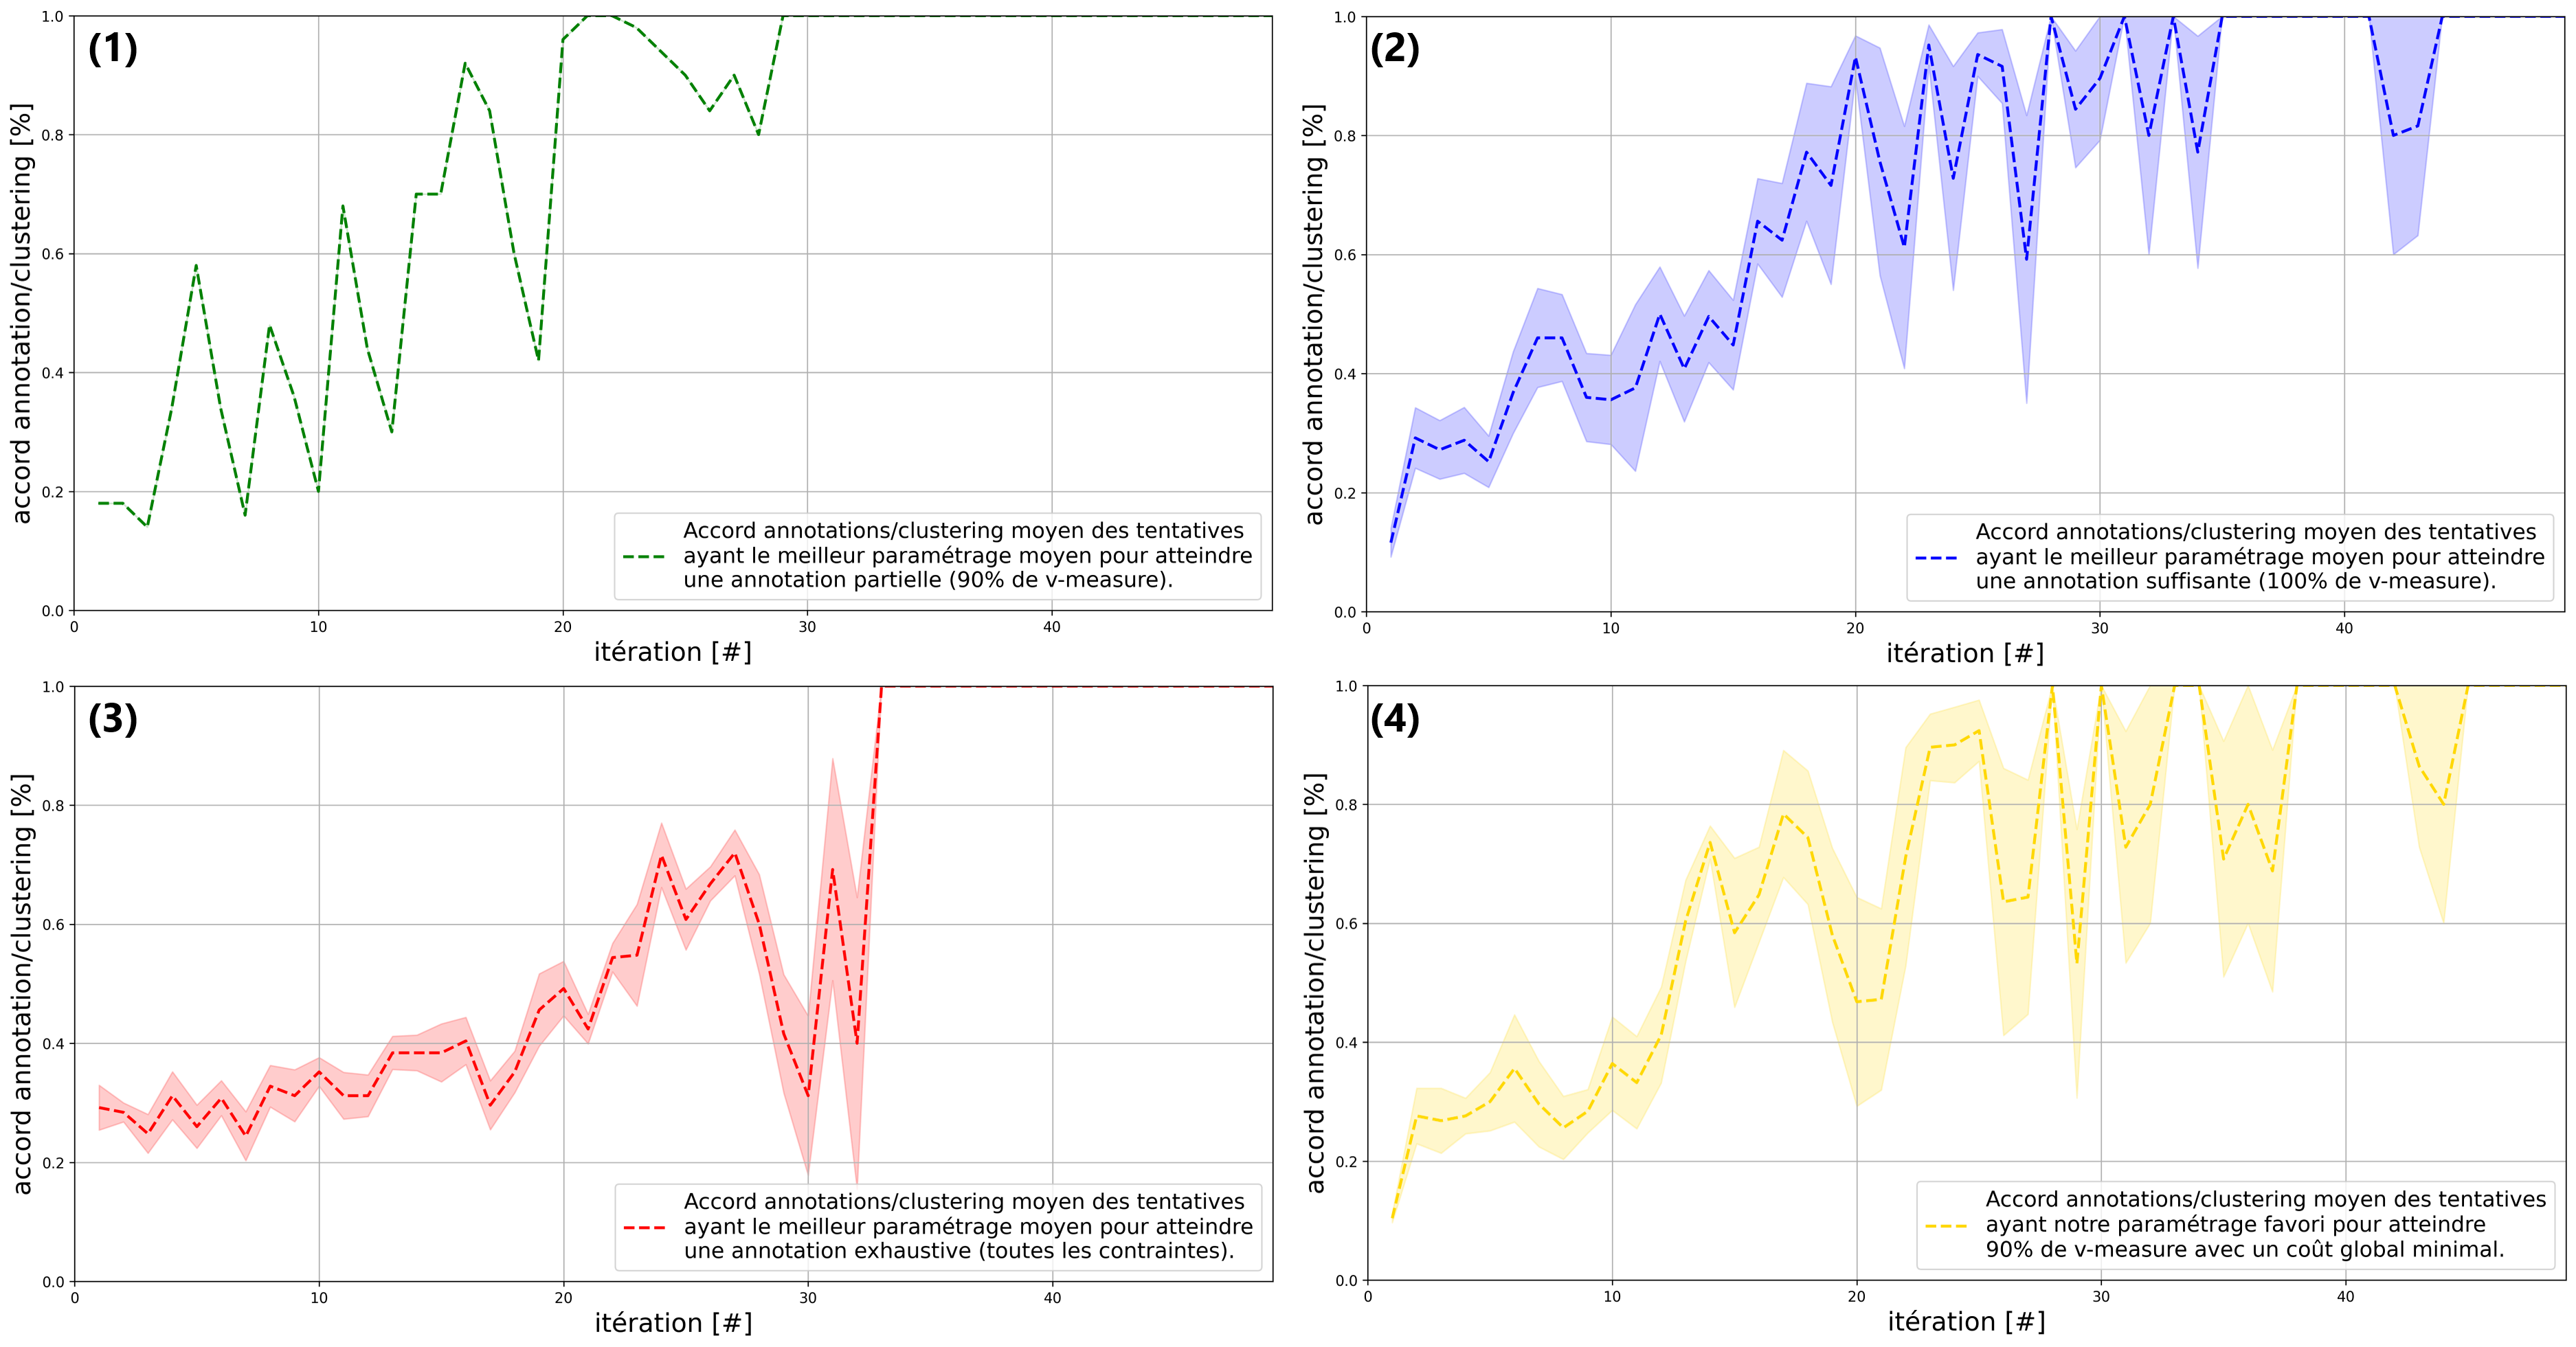
\includegraphics[width=0.95\textwidth]{figures/etude-rentabilite-accord-annotation}
				\caption{
					Évolution au cours des itérations de l'accord entre l'annotation de contraintes d'un expert et le résultat de \textit{clustering} sur lequel est basé l'échantillonnage de contraintes.
					Ces accords sont exprimés grâce à des lots de $50$ contraintes annotées.
					Les évolutions moyennes de différents paramétrages de la méthode sont exposées :
					\textbf{(1)} meilleur paramétrage moyen pour atteindre une annotation partielle ;
					\textbf{(2)} meilleur paramétrage moyen pour atteindre une annotation suffisante ;
					\textbf{(3)} meilleur paramétrage moyen pour atteindre une annotation exhaustive ;
					et \textbf{(4)} paramétrage favori.
					À titre d'information, les courbes en noir représentent l'évolution de la \texttt{v-measure} entre le \textit{clustering} et la vérité terrain.
				} 
				\label{figure:4.5.1-ETUDE-RENTABILITE-ACCORD-ANNOTATION-CLUSTERING}
			\end{figure}
			
			% Tableau : corrélation modérée.
			La \textsc{Table~\ref{table:4.5.1-ETUDE-RENTABILITE-CORRELATION-ACCORD-PERFORMANCE}} contient le score de corrélation entre cet accord et la performance théoriques obtenue grâce à la vérité terrain.
			Cette corrélation est modérée : $0.49$ sur l'ensemble des tentatives, $0.69$ sur les tentatives utilisant notre paramétrage favori.
			\begin{table}[!htb]
				\begin{center}
				\begin{tabular}{|c|r|}
				
					\hline
					% ENTETE DU TABLEAU
					\multicolumn{1}{|c|}{\shortstack[c]{
						Paramétrage
					}}
						& \multicolumn{1}{c|}{\shortstack[c]{
							Corrélation \texttt{r}
						}}
						\tabularnewline
						\hline
					
					% Annotation partielle.
					Meilleur paramétrage moyen pour une annotation partielle \textbf{(1)}
						& $0.92$
						\tabularnewline
						\hline
					
					% Annotation suffisante.
					Meilleur paramétrage moyen pour une annotation suffisante \textbf{(2)}
						& $0.74$
						\tabularnewline
						\hline
					
					% Annotation exhaustive.
					Meilleur paramétrage moyen pour une annotation exhaustive \textbf{(3)}
						& $0.57$
						\tabularnewline
						\hline
					
					% Paramétrage favori
					Paramétrage favori \textbf{(4)}
						& $0.69$
						\tabularnewline
						\hline
					
					% Moyenne des $960$ tentatives.
					Moyenne des $960$ tentatives
						& $0.49$
						\tabularnewline
						\hline
					
				\end{tabular}
				\end{center}
				\caption{
					Score de corrélation \texttt{r} de \textit{Pearson} entre la performance du \textit{clustering} obtenu à l'aide d'une vérité terrain (\texttt{v-measure}) et le score d'accord entre annotation et \textit{clustering}.
				}
				\label{table:4.5.1-ETUDE-RENTABILITE-CORRELATION-ACCORD-PERFORMANCE}
			\end{table}
			
			% Description de la figure : croissance instable.
			Cependant, la tendance constatée est aussi saccadée par de nombreux pics pouvant faire perdre ou gagner jusqu'à $40$\% d'accord entre deux itérations.
			Des chutes d'accord peuvent intervenir à des itérations où la similarité du \textit{clustering} avec la vérité terrain est pourtant forte, comme c'est le cas autour des itérations $29$ et $36$ où l'accord chute de plus de $25$\% alors que la \texttt{v-measure} avec la vérité terrain est constamment au dessus de de $95$\%.
			
			% Description de la figure : autres paramétrages
			Les autres paramétrages représentés dans \textbf{(1)}, \textbf{(2)} et \textbf{(3)} comportent des tendances similaires (corrélation forte mais variations soudaines d'accord, chute d'accords malgré des \textit{clustering} aux performances élevées, ...).

		%%% Discussion
		\subsubsection{Discussion}
		
			% Rappel de l'objectif : trouver un cas d'arrêt en regardant l'accord entre l'annotation et le clustering.
			Dans cette étude, nous avons analysé l'évolution de l'accord entre les annotations et le partitionnement de données proposé par un \textit{clustering} dans l'espoir de définir un cas d'arrêt de notre méthodologie d'annotation qui soit indépendant d'une vérité terrain pré-établie.
			Cependant, en considérant les résultats obtenus, ce score d'accord ne semble pas répondre à cette objectif.
			
			% Trop instable pour définir un cas d'arrêt.
			Tout d'abord, malgré une corrélation acceptable avec la performance théorique du \textit{clustering} (moyenne à $0.49$, voir \textsc{Table~\ref{table:4.5.1-ETUDE-RENTABILITE-CORRELATION-ACCORD-PERFORMANCE}}), l'évolution du score d'accord reste instable.
			En effet, les nombreuses variations et saccades rendent toute analyse de rentabilité difficile voire impossible, ce qui ne permet pas de définir un cas d'arrêt pour notre méthode d'annotation.
			
			\begin{leftBarExamples}
				Concernant l'évolution du paramétrage favori (\textsc{Figure~\ref{figure:4.5.1-ETUDE-RENTABILITE-ACCORD-ANNOTATION-CLUSTERING}} \textbf{(4)}), nous ne pouvons pas précisément définir à partir de quelle itération les résultats semblent intéressant car le score d'accord oscille longuement entre $50$\% et $100$\% avec des pics de plus de $25$\% entre deux itérations. 
			\end{leftBarExamples}
			
			\begin{leftBarAuthorOpinion}
				% Rappel: l'objectif de notre méthode d'annotation est de corriger le plus rapidement un clustering.
				Après réflexion, ce score d'accord est probablement infructueux à cause du fonctionnement même de notre méthode, dont l'objectif est de corriger le partitionnement des données en utilisant un minimum de contraintes.
				En effet, dans le cadre de l'optimisation des paramètres réalisée en \textsc{Section~\ref{section:4.2-HYPOTHESE-EFFICIENCE}}, nous avons retenu dans notre paramétrage favori la sélection des contraintes les plus proches entre deux \textit{clusters} différents (\texttt{samp.closest.diff}) : cette sélection permet ainsi de décrire efficacement l'emplacement des frontières de \textit{clusters}.
				
				% Cet échantillonnage est non supervisé : il y a de nombreuses saccades.
				Or, cet échantillonnage reste une méthode non-supervisée : aux premières itérations, les contraintes sélectionnées ont de bonnes chances de mettre en avant une frontière mal positionnée, mais au fur et à mesure que des contraintes s'ajoutent, les nouvelles contraintes ont moins de chances de trouver des bordures de \textit{clusters} qui ne soient pas encore caractérisées.
				De ce fait, il se peut que les dernières sélections n'identifient aucune nouvelle frontière, qu'elles se concentrent sur des frontières déjà bien positionnées ou déjà décrites par d'autres contraintes, ou qu'elles nécessitent plusieurs itérations pour caractériser des frontières complexes (le comportement des autres méthodes de sélections représentées en \textsc{Figure~\ref{figure:4.5.1-ETUDE-RENTABILITE-ACCORD-ANNOTATION-CLUSTERING}} peut être illustré par des raisonnements similaires).
				L'ensemble de ces cas de figures peut ainsi expliquer les nombreuses saccades dans l'évolution du score d'accord : tantôt la sélection semble pertinente, tantôt la sélection semble inutile.
			\end{leftBarAuthorOpinion}
			
			% Trop instable pour caratériser une itération.
			Pour aller plus loin, nous pouvons aussi critiquer le score de corrélation qui ne semble pas montrer de lien fort entre les performances théoriques et les accords calculés, tant sur l'ensemble des tentatives que pour le paramétrage favori.
			Il est même rare d'observer des chutes importantes d'accords qui soient accompagnées d'une variation significative de \texttt{v-measure} avec la vérité terrain.
			Au final, ce score d'accord n'est donc pas vraiment représentatif de la rentabilité d'une itération ou de l'évolution de la pertinence du \textit{clustering}.
			\begin{leftBarAuthorOpinion}
				Pour expliquer cette absence de corrélation, il est possible que l'analyse des annotations réalisées ait été une idée infructueuse : les $50$ contraintes annotées peuvent peut-être exprimer un désaccord avec le précédent \textit{clustering}, mais ce n'est pas pour autant que l'ajout de ces nouvelles contraintes impacte significativement la pertinence globale du partitionnement des données.
			\end{leftBarAuthorOpinion}
			
			% Conclusions et suggestion.
			En conclusion, \textbf{le score d'accord entre l'annotation courante et le \textit{clustering} précédent n'est pas adéquat pour estimer un cas d'arrêt de notre méthode d'annotation}, principalement car il est trop instable et qu'il ne représente pas bien les bénéfices obtenus à chaque itération.
			Ainsi, si une analyse de l'annotation réalisée n'est pas fructueuse, nous nous tournerons vers l'analyse plus abstraite des différences entre deux résultats de \textit{clustering}
	
	%%%
	%%% Subsection 4.5.2: Étude de l'évolution de la différence entre deux \textit{clusterings} consécutifs.
	%%%
	\subsection{Étude de l'évolution de la différence entre deux \textit{clusterings} consécutifs}
	\label{section:4.5.2-ETUDE-RENTABILITE-SIMILARITE-CLUSTERING}
		
		% Objectif de l'expérience.
		Nous venons de conclure que l'analyse de l'accord entre l'annotation et le partitionnement des données ne permet pas d'estimer la rentabilité d'une itération de notre méthode d'annotation.
		Parmi les explications possibles, nous avons mis en cause l'analyse du lot de contraintes annotées : en effet, ce n'est pas parce que l'annotation de contraintes est en désaccord avec le précédent partitionnement des données que les correctifs associés auront un impact significatif sur le prochain partitionnement.
		Ainsi, nous voulons analyser l'évolution de la différence entre deux \textit{clusterings} successifs : en effet, si une itération apporte des correctifs ayant un impact, alors il devrait y avoir des différences visibles entre les deux itérations de \textit{clustering}.
	
		%%% Protocole expérimental.
		\subsubsection{Protocole expérimental}
			
			% Axiome.
			\begin{leftBarWarning}
				Dans le cadre de cette étude, nous supposons que l'expert métier connaît parfaitement le domaine traité dans ce jeu de données, et qu'il est capable de caractériser sans ambiguïté la similitude entre deux données issues de cet ensemble.
			\end{leftBarWarning}
			
			% Pseudo-code.
			Pour résumer le protocole expérimental que nous décrivons ci-dessous, vous pouvez vous référer au pseudo-code décrit dans \textsc{Algorithme~\ref{algorithm:4.5.1-ETUDE-RENTABILITE-SIMILARITE-CLUSTERING-PROTOCOLE}}.
			
			\begin{algorithm}
				\KwData{jeu de données annotés (vérité terrain)}
				%
				\ForEach{jeux de données à tester}{
					\textbf{initialisation (données)}: récupérer les données et la vérité terrain \;
					\textbf{initialisation (contraintes)}: créer une liste vide de contraintes \;
					\textbf{prétraitement}: supprimer le bruit dans les données avec \texttt{prep.simple} \;
					\textbf{vectorisation}: transformer les données en vecteurs avec \texttt{vect.tfidf} \;
					\textbf{clustering initial}: regrouper les données par similarité avec \texttt{clust.kmeans.cop} \;
					\Repeat{annotation de toutes les contraintes possibles}{
						\textbf{échantillonnage}: sélectionner des contraintes avec \texttt{samp.closest.diff} \;
						\textbf{simulation d'annotation}: caractériser les contraintes grâce à la vérité terrain \;
						\textbf{intégration}: ajouter les nouvelles contraintes au gestionnaire de contraintes \;
						\textbf{clustering}: regrouper les données par similarité avec \texttt{clust.kmeans.cop} \;
						\textbf{rentabilité}: calculer la différence entre les deux précédents \textit{clusterings} \;
					}
				}
				\textbf{analyse 1}: afficher l'évolution de la différence entre deux \textit{clustering} consécutifs \;
				\textbf{analyse 2}: calculer la corrélation entre le score de différence et le score de performance \;
				%
				\KwResult{discussion sur la rentabilité d'après la différence entre \textit{clusterings}}
				%
				\caption{\textit{
					Description en pseudo-code du protocole expérimental de l'étude de l'évolution de la différence entre deux \textit{clustering} consécutifs.
				}}
				\label{algorithm:4.5.1-ETUDE-RENTABILITE-SIMILARITE-CLUSTERING-PROTOCOLE}
			\end{algorithm}

			% Détails de l'expérience.
			Nous nous appuyons sur le même protocole que l'expérience précédente (cf. \textsc{Section~\ref{section:4.5.1-ETUDE-RENTABILITE-ACCORD-ANNOTATION-CLUSTERING}}) : nous utilisons comme vérité terrain le jeu de données \texttt{Bank Cards (v1.0.0)}, nous réalisons $5$ tentatives complètes de la méthode du \textit{clustering} interactif en utilisant notre paramétrage favori, et nous simulons l'annotation par un expert d'un lot de $50$ contraintes à chaque itération.
			
			% Ajout de la comparaison entre clustering.
			Cependant, au lieu de calculer un score d'accord entre annotation et \textit{clustering}, nous estimons la différence entre le \textit{clustering} précédent et le \textit{clustering} obtenu grâce aux dernières annotations.
			Cette différence entre deux \textit{clustering} $X$ et $Y$ est obtenue par la formule $1-\texttt{v-measure}(X,Y)$ où la \texttt{v-measure} caractérise la ressemblance entre deux partitionnements des données (\cite{rosenberg-hirschberg:2007:vmeasure-conditional-entropybased}).
			Pour nous permettre de discuter de l'utilité de ce score pour prédire la stabilisation du \textit{clustering} et ainsi définir un cas d'arrêt de notre méthodologie d'annotation, nous calculons aussi le score de corrélation entre cette différence et la performance obtenue à l'aide d'une vérité terrain (la corrélation \texttt{r} de \textit{Pearson} (\cite{kirch:2008:pearson-correlation-coefficient}) est utilisée).
			
			\begin{leftBarIdea}
				Comme précédemment, nous concentrons l'étude sur notre paramétrage favori (voir \textsc{Section~\ref{section:4.4.3-ETUDE-PERTINENCE-RESUME-AUTOMATIQUE}}).
				Cependant, afin de compléter notre discussion avec d'autres points de comparaison, nous analysons aussi les autres paramétrages implémentés, notamment les meilleurs paramétrages moyens identifiés lors de l'hypothèse d'efficience (voir \textsc{Section~\ref{section:4.2-HYPOTHESE-EFFICIENCE}}).
			\end{leftBarIdea}
			
			% Référence scripts.
			\begin{leftBarInformation}
				Les scripts de l'expérience, réalisés avec des \textit{notebooks} Python (\cite{van-rossum-drake:2009:python-reference-manual}), sont disponibles dans un dossier dédié de~\cite{schild:2021:cognitivefactory-interactiveclusteringcomparativestudy}.
			\end{leftBarInformation}

		%%% Résultats
		\subsubsection{Résultats obtenus}
			
			% Figure : décroissance générale.
			La \textsc{Figure~\ref{figure:4.5.2-ETUDE-RENTABILITE-SIMILARITE-CLUSTERING}} représente l'évolution moyenne du score de différence entre deux \textit{clusterings} pour les quatre paramétrages mis en avant lors de nos études.
			Nous pouvons constater une tendance générale à la décroissance vers $0$\% de ce score de différence : pour le paramétrage favori, la différence moyenne entre deux \textit{clustering} est initialement comprise entre $25$\% et $35$\% jusqu'à l'itération $10$, elle chute ensuite pour être inférieure à $5$\% après l'itération $20$, et elle termine enfin en oscillant très légèrement ($\pm1$\%) autour de $0$\% jusqu'à la fin des annotations.
			\begin{figure}[!htb]
				\centering
				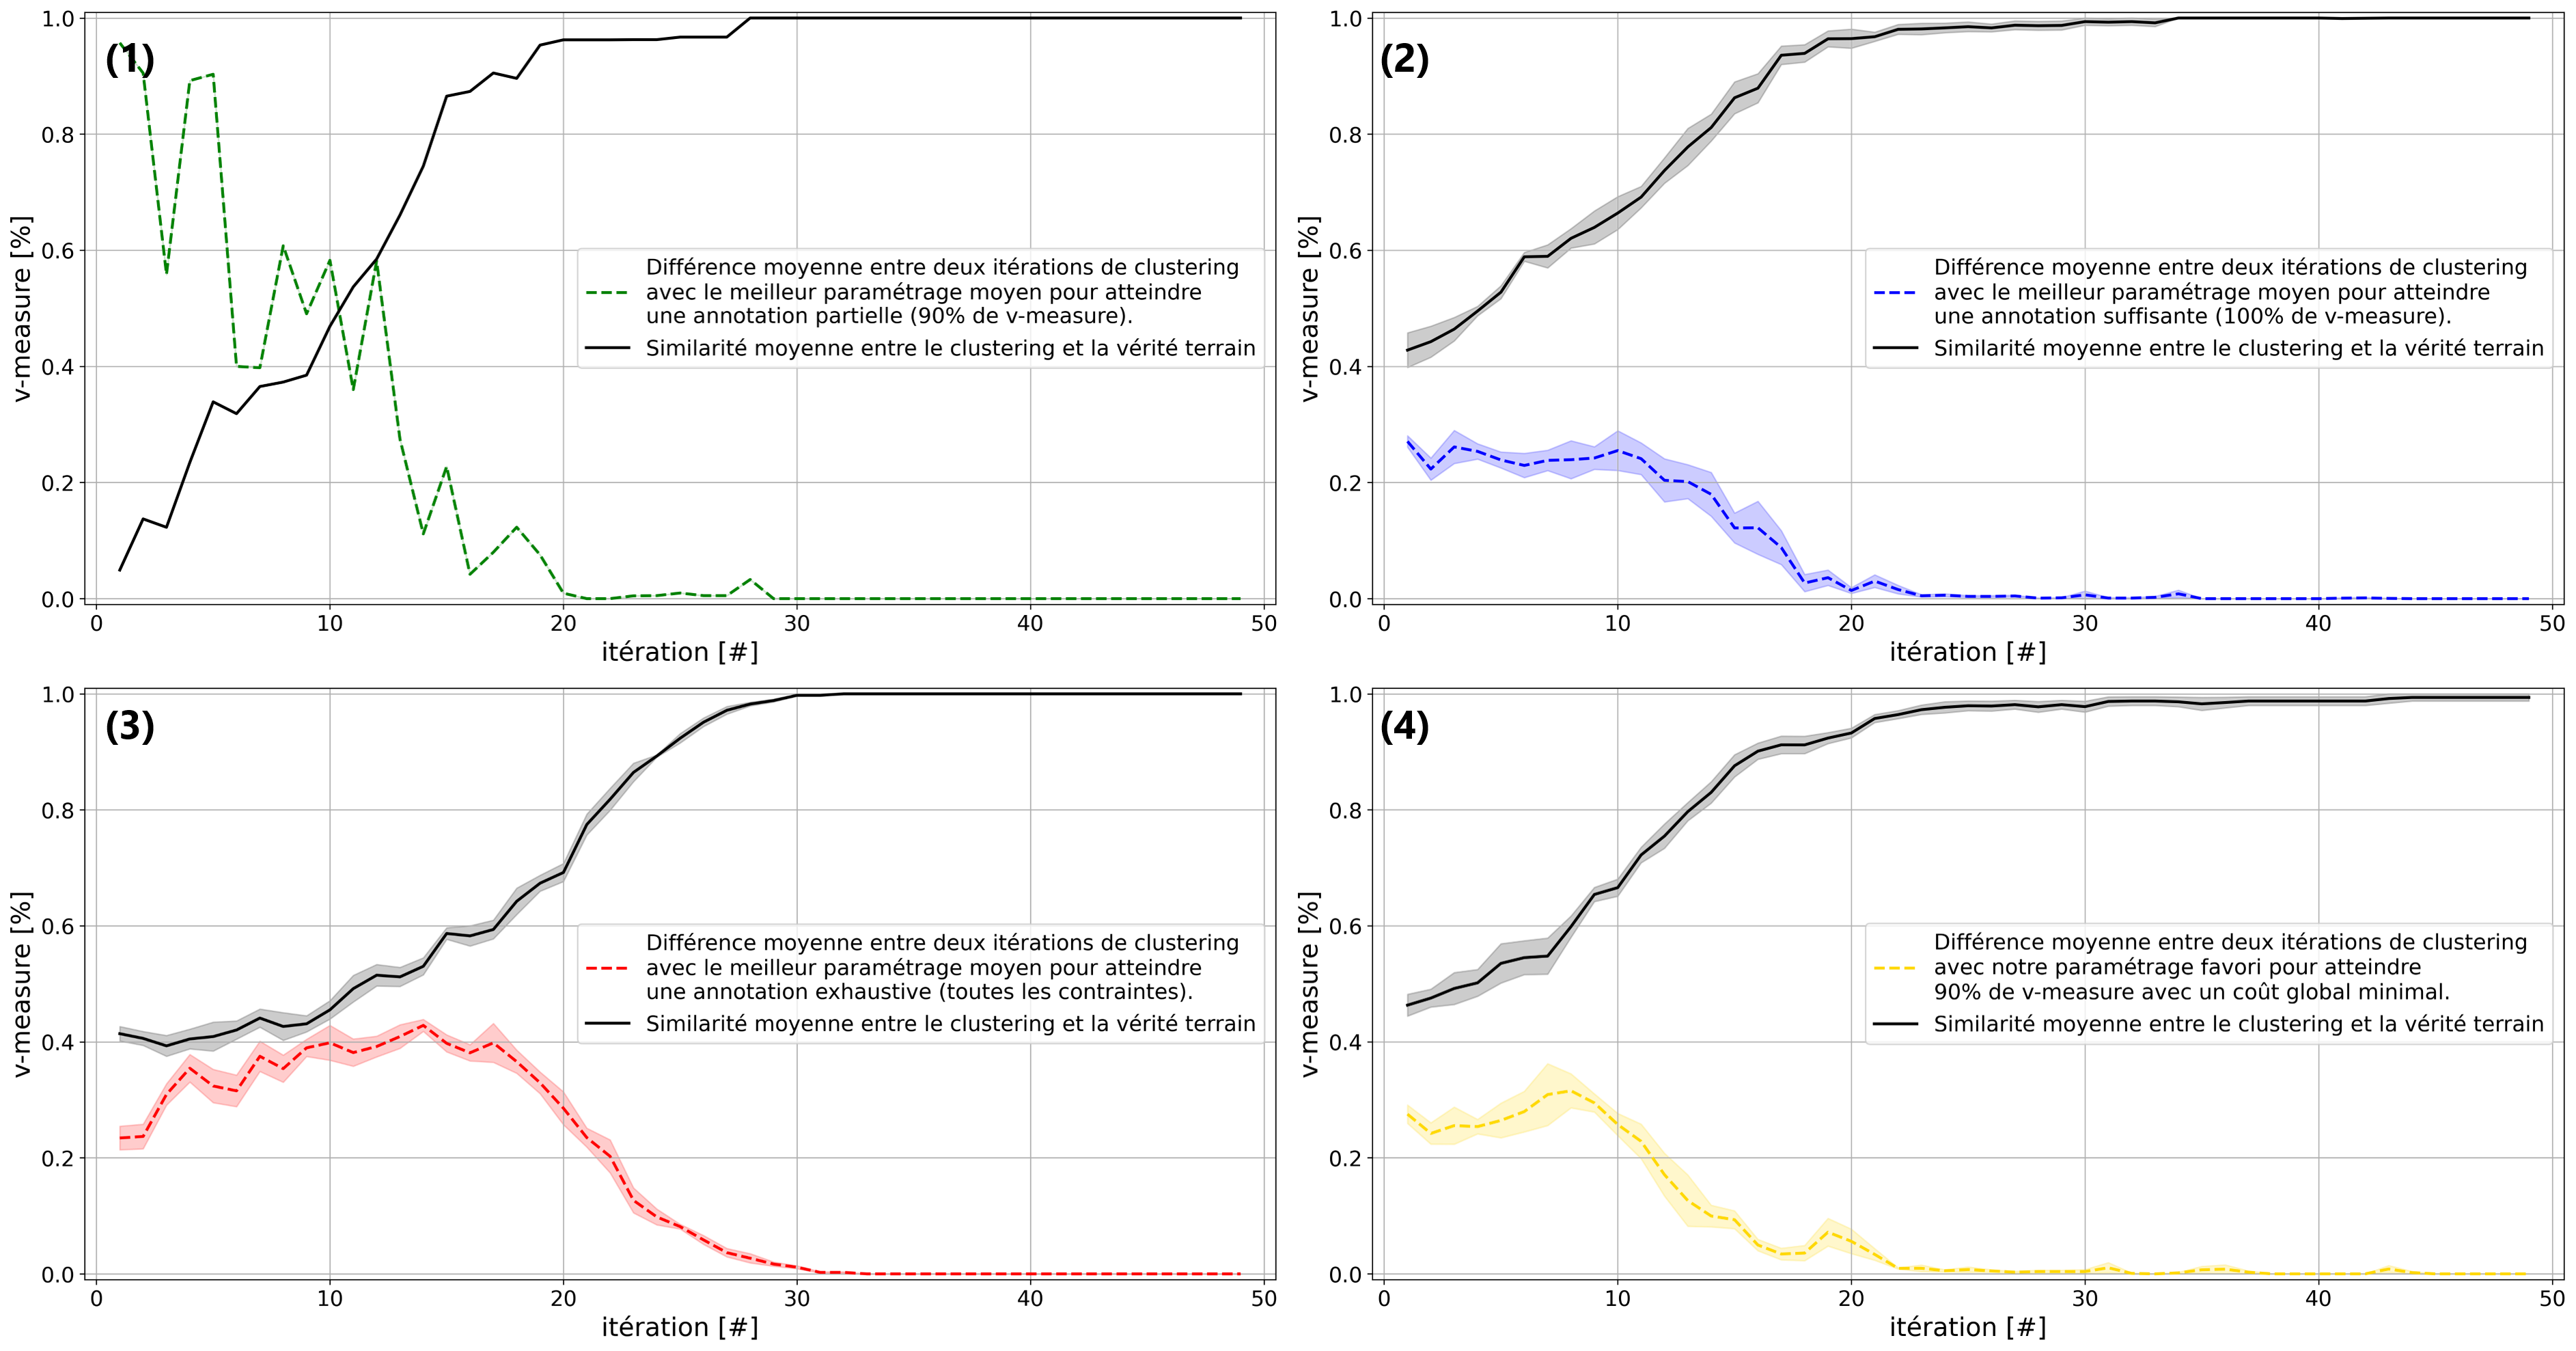
\includegraphics[width=0.95\textwidth]{figures/etude-rentabilite-similarite-clustering}
				\caption{
					Évolution de la différence de résultats entre deux itérations de \textit{clustering}.
					Les évolutions moyennes de différents paramétrages de la méthode sont exposées :
					\textbf{(1)} meilleur paramétrage moyen pour atteindre une annotation partielle ;
					\textbf{(2)} meilleur paramétrage moyen pour atteindre une annotation suffisante ;
					\textbf{(3)} meilleur paramétrage moyen pour atteindre une annotation exhaustive ;
					et \textbf{(4)} paramétrage favori.
					À titre d'information, les courbes en noir représentent l'évolution de la \texttt{v-measure} entre le \textit{clustering} et la vérité terrain.
				}
				\label{figure:4.5.2-ETUDE-RENTABILITE-SIMILARITE-CLUSTERING}
			\end{figure}
			
			% Tableau : corrélation forte.
			La \textsc{Table~\ref{table:4.5.2-ETUDE-RENTABILITE-CORRELATION-SIMILARITE-PERFORMANCE}} contient le score de corrélation entre cette différence et la performance théoriques obtenue grâce à la vérité terrain.
			Cette corrélation est forte : $0.75$ sur l'ensemble des tentatives, $0.93$ sur les tentatives utilisant notre paramétrage favori.
			La \textsc{Figure~\ref{figure:4.5.2-ETUDE-RENTABILITE-SIMILARITE-CLUSTERING}} confirme cette corrélation :
			\begin{itemize}
				\item un score de \texttt{v-measure} avec la vérité terrain proche de $100$\% est accompagné d'un score de différence proche de $0$\% (après l'itération $20$ pour \textbf{(1)}, après l'itération $20$ pour \textbf{(2)}, après l'itération $30$ pour \textbf{(3)} et après l'itération $22$ pour \textbf{(4)}) ;
				\item une croissance de performance est généralement accompagnée d'un score non nul de différence (voir \textbf{(2)} et \textbf{(4)} entre les itérations $0$ et $20$), et plusieurs pics de performance sont accompagnés de scores forts de différence (particulièrement visible sur \textbf{(1)} vers l'itération $5$ et entre les itérations $10$ et $15$) ;
				\item il est toutefois à noter que l'inverse n'est pas vrai : un score non nul de différence n'accompagne pas forcément une croissance de performance, mais peut simplement caractériser un changement de partitionnement, comme c'est le cas dans \textbf{(3)} entre les itérations $0$ et $10$ où des modifications ont lieu (score de différence non nul) mais où la performance par rapport à la vérité terrain stagne.
			\end{itemize}
			\begin{table}[!htb]
				\begin{center}
				\begin{tabular}{|c|r|}
				
					\hline
					% ENTETE DU TABLEAU
					\multicolumn{1}{|c|}{\shortstack[c]{
						Paramétrage
					}}
						& \multicolumn{1}{c|}{\shortstack[c]{
							Corrélation
						}}
						\tabularnewline
						\hline
					
					% Annotation partielle.
					Meilleur paramétrage moyen pour une annotation partielle \textbf{(1)}
						& $0.96$
						\tabularnewline
						\hline
					
					% Annotation suffisante.
					Meilleur paramétrage moyen pour une annotation suffisante \textbf{(2)}
						& $0.92$
						\tabularnewline
						\hline
					
					% Annotation exhaustive.
					Meilleur paramétrage moyen pour une annotation exhaustive \textbf{(3)}
						& $0.85$
						\tabularnewline
						\hline
					
					% Paramétrage favori
					Paramétrage favori \textbf{(4)}
						& $0.93$
						\tabularnewline
						\hline
					
					% Moyenne des $960$ tentatives.
					Moyenne des $960$ tentatives
						& $0.75$
						\tabularnewline
						\hline
					
				\end{tabular}
				\end{center}
				\caption{
					Score de corrélation \texttt{r} de \textit{Pearson} entre la performance du \textit{clustering} obtenu à l'aide d'une vérité terrain (\texttt{v-measure}) et le score de différence entre deux \textit{clusterings} consécutifs.
				}
				\label{table:4.5.2-ETUDE-RENTABILITE-CORRELATION-SIMILARITE-PERFORMANCE}
			\end{table}
			
			% Description de la figure : autres paramétrages
			Les autres paramétrages représentés dans \textbf{(1)}, \textbf{(2)} et \textbf{(3)} comportent des tendances similaires (décroissance générale, forte corrélation avec la performance théorique) à quelques détails (\textbf{(1)} commence avec des scores de différence très forts avant décroître avec de nombreux pics ; \textbf{(3)} croît légèrement avant d'entamer sa décroissance, ...).
			
		%%% Discussion
		\subsubsection{Discussion}
		
			% Rappel de l'objectif : trouver un cas d'arrêt en regardant l'évolution de la différence entre deux clusterings.
			Dans cette étude, nous avons analysé l'évolution du score de différence entre deux itérations de \textit{clustering} dans l'espoir de définir un cas d'arrêt de notre méthodologie d'annotation qui soit indépendant d'une vérité terrain pré-établie.
			
			% Avantage 1 : Caractérise la rentabilité.
			Tout d'abord, nous pouvons affirmer qu'il y une forte corrélation entre l'évolution de ce score de différence et l'évolution du score de performance (voir \textsc{Table~\ref{table:4.5.2-ETUDE-RENTABILITE-CORRELATION-SIMILARITE-PERFORMANCE}} : \texttt{r} moyen de $0.75$ ; \texttt{r} supérieur à $0.85$ pour les paramétrages mis en avant).
			Cette corrélation est confirmée visuellement grâce à la \textsc{Figure~\ref{figure:4.5.2-ETUDE-RENTABILITE-SIMILARITE-CLUSTERING}} : plus les différences entre \textit{clusterings} sont faibles, plus les performances des \textit{clusterings} sont fortes.
			
			% Attention : Peut ne caractériser qu'un gros changement sans pour autant une amélioration.
			Un point d'attention est toutefois à retenir : une modification du partitionnement des données n'entraîne pas forcément un gain de performance (voir \textbf{(3)} entre les itérations $0$ et $10$ et \textbf{(4)} entre les itérations $0$ et $8$).
			Nous ne pouvons donc pas conclure que l'analyse de la différence entre eux itération de \textit{clustering} permet de caractériser totalement la rentabilité d'une itération.
			
			% Avantage 2 : Permet de définir un cas d'arrêts.
			Cependant, nous pouvons tout de même nous servir de ce score pour définir un cas d'arrêt pour notre méthodologie d'annotation lorsque la différence entre deux \textit{clusterings} est faible.
			Pour cela, il nous suffit de fixer un seuil bas du score de différence en dessous duquel il n'est plus rentable de faire de nouvelles itérations de la méthode car les performances devraient être suffisantes.
			Une analyse manuelle ou semi-manuelle (voir hypothèse de pertinence en \textsc{Section~\ref{section:4.4-HYPOTHESE-PERTINENCE}}) reste nécessaire pour confirmer la valeur métier du résultat obtenu.
			
			\begin{leftBarIdea}
				Si nous restons sur notre seuil théorique de $90$\% de \texttt{v-measure} (voir \textsc{Section~\ref{section:4.2-HYPOTHESE-EFFICIENCE}}) et que nous nous basons sur la \textsc{Figure~\ref{figure:4.5.2-ETUDE-RENTABILITE-SIMILARITE-CLUSTERING}} \textbf{(4)}, nous pouvons visuellement fixer ce seuil autour de $5$\% de différences.
				Le réglage fin de ce seuil pourra être le sujet de futures analyses complémentaires.
			\end{leftBarIdea}
			
			% Conclusions et suggestion.
			En conclusion, \textbf{le score de différences entre deux résultats de \textit{clustering} semble être un bon indicateur pour estimer un cas d'arrêt de notre méthodologie d'annotation}, et nous proposer d'utiliser un seuil de $5$\% pour implémenter ce cas d'arrêt.
			
	%%%
	%%% Subsection 4.5.3: Mise en commun des stratégies d'évaluation de la rentabilité d'une itération de la méthode et définition d'un cas d'arrêt indépendant d'une vérité terrain.
	%%%
	\subsection{Mise en commun des stratégies d'évaluation de la rentabilité d'une itération de la méthode et définition d'un cas d'arrêt indépendant d'une vérité terrain.}
	\label{section:4.5.3-ETUDE-RENTABILITE-MISE-EN-COMMUN}
			
		% Conclusion.
		\begin{leftBarSummary}
			Au cours de cette étude de rentabilité, nous avons pu voir que :
			\begin{itemize}
				\item[\itemko] l'analyse du score d'accord entre l'annotation courante et le \textit{clustering} précédent ne permet pas d'estimer la rentabilité d'une itération, ni de définir un cas d'arrêt de notre méthodologie d'annotation (cf. \textsc{Section~\ref{section:4.5.1-ETUDE-RENTABILITE-ACCORD-ANNOTATION-CLUSTERING}}) ;
				\item[\itemok] l'analyse des différences entre deux itérations de \textit{clusterings} est une approche prometteuse pour estimer la rentabilité d'une itération, bien qu'une modification significative entre deux résultats de \textit{clustering} n'implique pas forcément un gain de performance (les deux \textit{clustering} peuvent avoir une \texttt{v-measure} équivalente avec la vérité terrain) ;
				\item[\itemok] l'usage de différences entre deux itérations de \textit{clusterings} permet de définir un cas d'arrêt de de notre méthodologie d'annotation : si les différences sont faibles (par exemple : inférieures à $5$\%), alors les performances stagnent ou plafonnent, donc il peut être intéressant d'interrompre le \textit{clustering} interactif après avoir vérifier la manuellement pertinence des résultats obtenus (cf. (cf. \textsc{Section~\ref{section:4.5.2-ETUDE-RENTABILITE-SIMILARITE-CLUSTERING}}) et \textsc{Section~\ref{section:4.4.4-ETUDE-PERTINENCE-MISE-EN-COMMUN}}).
			\end{itemize}
		\end{leftBarSummary}
		
		% Transition: Vers Simulation d'erreurs.
		Pour terminer nos différentes analyses, il convient maintenant d'anticiper la présence d'erreurs d’annotation.
		En effet, nous avons fait jusqu'à présent l'hypothèse que l'annotateur ne se trompe jamais, mais cette hypothèse forte n'est pas toujours vérifiée en pratique.
		Pour estimer l'impact de ces erreurs ou incohérences d'annotation, nous devons donc réaliser une analyse de robustesse de notre méthode d'annotation : celle-ci sera réalisé en \textsc{Section~\ref{section:4.6-HYPOTHESE-ROBUSTESSE}}.